\part{Pathfinding}
\frame{\partpage}

\begin{frame}{The problem}
    \begin{itemize}
        \item We have a \textbf{graph} \pause
            \begin{itemize}
                \item \textbf{Nodes} (points) \pause
                \item \textbf{Edges} (lines between points, each with a \textbf{length}) \pause
            \end{itemize}
        \item E.g.\ a road map \pause
            \begin{itemize}
                \item Nodes = addresses \pause
                \item Edges = roads \pause
            \end{itemize}
        \item E.g.\ a tile-based 2D game \pause
            \begin{itemize}
                \item Nodes = grid squares \pause
                \item Edges = connections between adjacent squares \pause
            \end{itemize}
        \item Given two nodes $A$ and $B$, find the \textbf{shortest path} from $A$ to $B$ \pause
            \begin{itemize}
                \item ``Shortest'' in terms of edge lengths --- could be distance, time, fuel cost, ...
            \end{itemize}
    \end{itemize}
\end{frame}

\begin{frame}{Applications of pathfinding}
    \begin{center}
        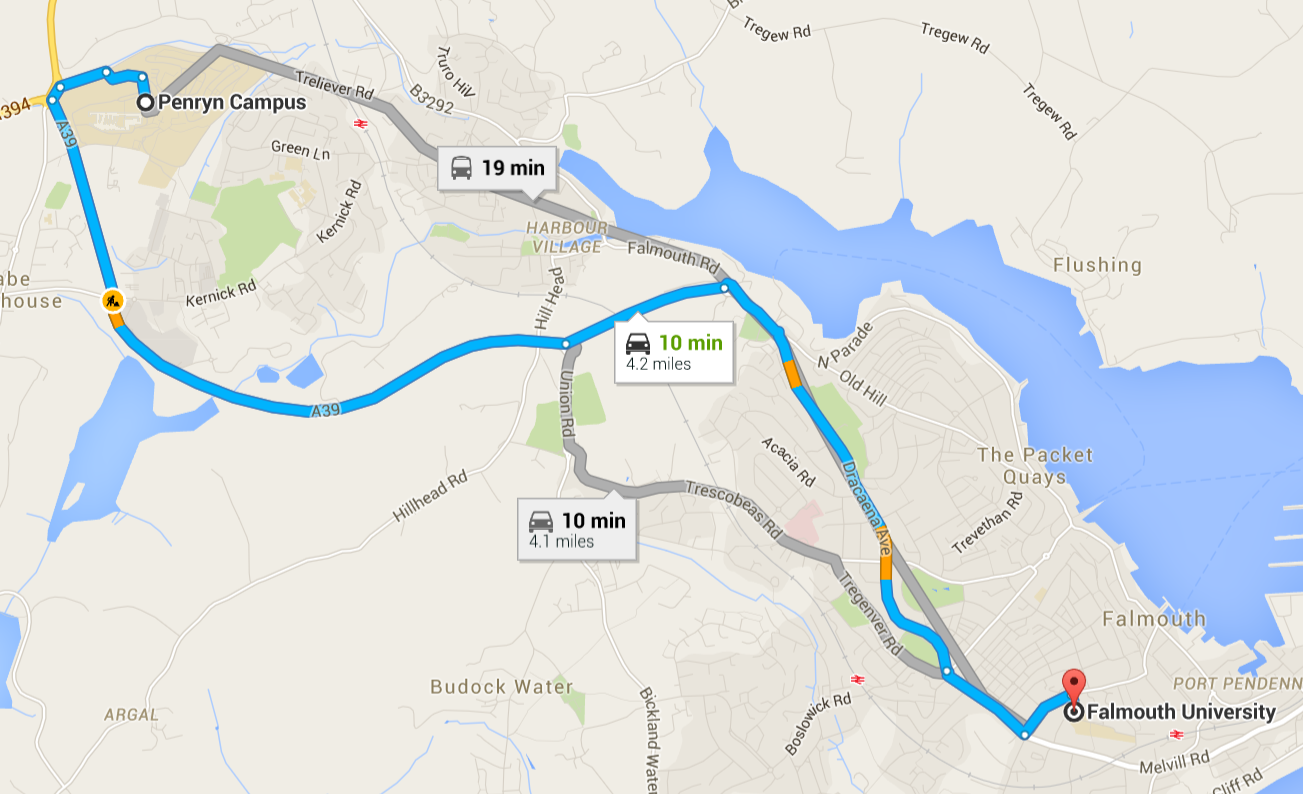
\includegraphics[width=\textwidth]{pathfinding_1}
    \end{center}
\end{frame}

\begin{frame}{Applications of pathfinding}
    \begin{center}
        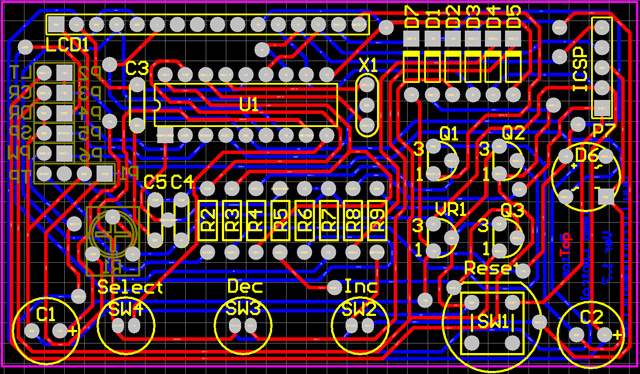
\includegraphics[width=\textwidth]{pcb}
    \end{center}
\end{frame}

\begin{frame}{Applications of pathfinding}
    Many applications in game AI \pause
    \begin{itemize}
        \item Non-player character AI \pause
        \item Mouse-based movement (e.g.\ strategy games) \pause
        \item Maze navigation \pause
        \item Puzzle solving
    \end{itemize}
\end{frame}

\begin{frame}{A$^*$ search}
    Idea: \pause
    \begin{itemize}
        \item Expand out from the start node \pause
        \item Let $g(n)$ be the length of the path currently found between the start and node $n$ \pause
        \item Let $h(n)$ be an \textbf{estimate} of the distance from $n$ to the goal \pause
        \item Prioritise nodes for which $g(n) + h(n)$ is small
    \end{itemize}
\end{frame}

\begin{frame}{Properties of A$^*$ search}
    \begin{itemize}
        \item A$^*$ is \textbf{guaranteed} to find the shortest path
            if the distance estimate is \textbf{admissible} \pause
        \item Essentially, \textbf{admissible} means it must be an \textbf{underestimate} \pause
            \begin{itemize}
                \item E.g.\ straight line Euclidean distance is clearly an underestimate
                    for actual travel distance \pause
            \end{itemize}
        \item A$^*$ is an example of \textbf{heuristic} search \pause
            \begin{itemize}
                \item In AI, a heuristic is an estimate based on human intuition \pause
                \item Heuristics are often used to prioritise search,
                    i.e.\ explore the most promising options first
            \end{itemize}
    \end{itemize}
\end{frame}

\begin{frame}{Implementing A$^*$}
    \begin{center}
        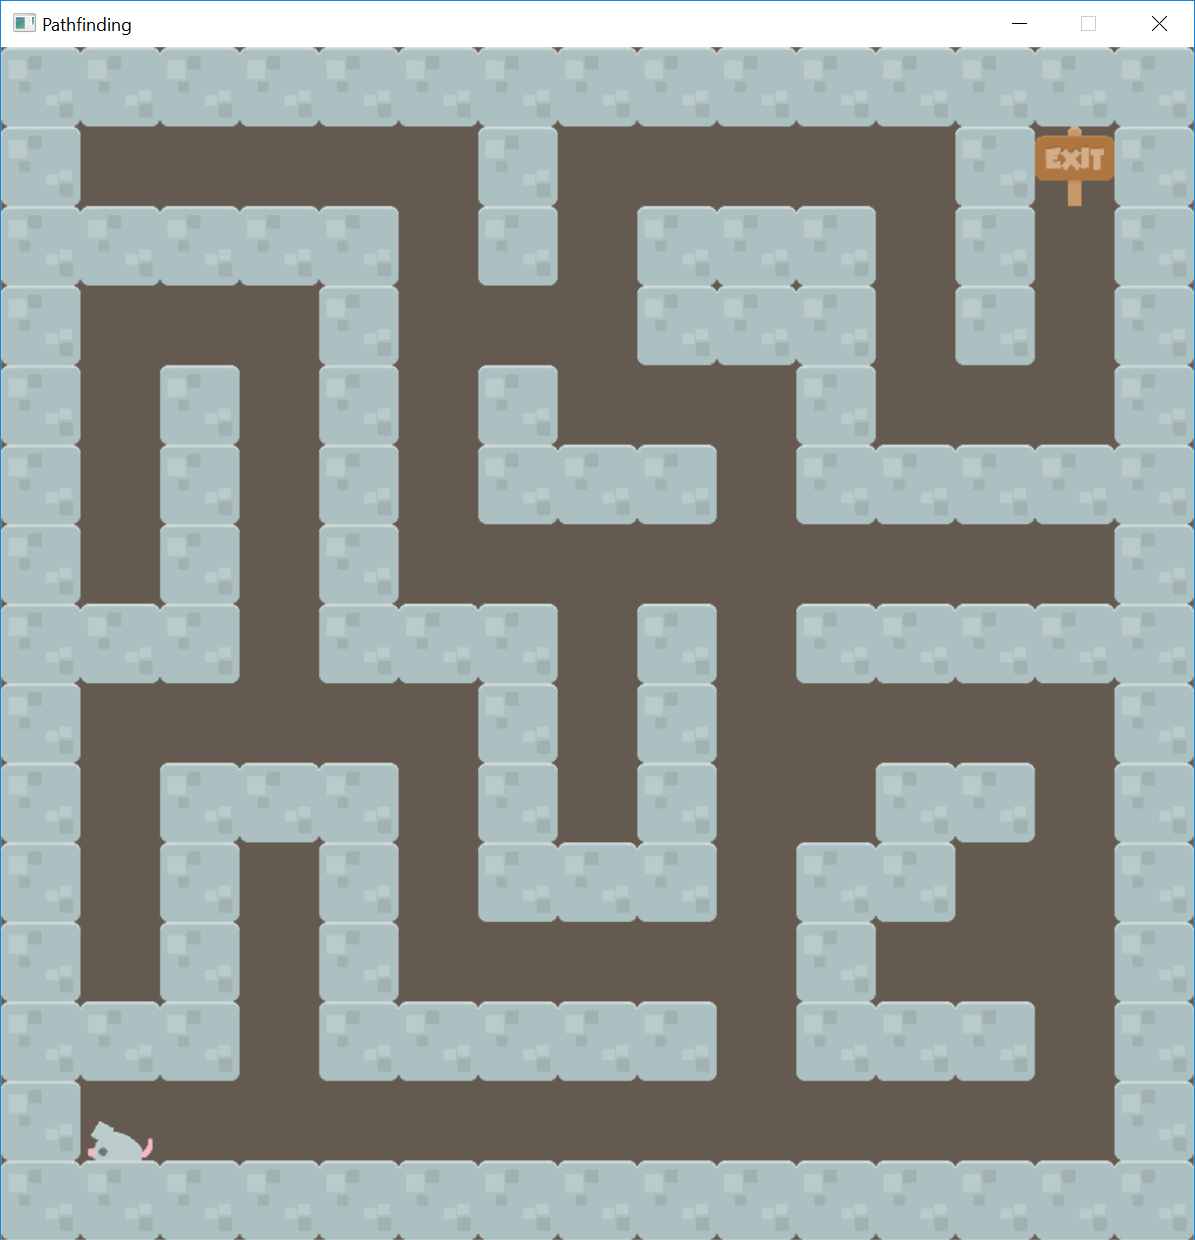
\includegraphics[width=0.4\textwidth]{application}
    \end{center}
    \begin{itemize}
        \item Worksheet 5 on LearningSpace
        \item Deadline: \textbf{9th March at 6pm} (i.e.\ two weeks from today)
    \end{itemize}
\end{frame}

